\documentclass[aspectratio=169]{beamer}
\usetheme{rulemancerlight}
\renewcommand{\rulemancerlogopath}{../logo.png}

\usepackage[T1]{fontenc}
\usepackage[utf8]{inputenc}
\usepackage{lmodern}
\usepackage{hyperref}
\usepackage{tikz}
\usetikzlibrary{arrows.meta,positioning}

\title{Rulemancer}
\subtitle{A CLIPS-based engine for rules-driven games}
\author{Mirko Mariotti}
\date{\today}

\begin{document}

\begin{frame}
  \titlepage
\end{frame}

\begin{frame}{What is and Why Rulemancer?}
\begin{center}

Rulemancer is a framework that allows you to define game logic in CLIPS rule files, while providing a Go-based server
to handle API interactions and transport. \\
\vspace{1cm}
Many game backends hard-code rules in application code. \\
Instead, Rulemancer separates \textbf{game logic} (CLIPS rules) from \textbf{transport/API} (Go server) and 
manages to rebuild games interfaces automatically. \\
\vspace{1cm}
This allows for:
\begin{itemize}
  \item Rapid prototyping of new games by writing CLIPS files.
  \item A unified interface for multiple games and room-based multiplayer.
\end{itemize}
\end{center}
\end{frame}

\begin{frame}{Project Snapshot}
\begin{itemize}
  \item Supports multiple games, rooms, and clients from a single server process.
  \vspace{0.4cm}
  \item Supports room-based multiplayer where each room:
  \vspace{0.4cm}
  \begin{itemize}
    \item Isolates game state in a separate CLIPS environment.
    \item Accepts player actions as CLIPS facts assertions via REST API.
    \item Processes game logic through CLIPS rules and returns results as structured responses.
    \item Processes queries to retrieve game state information.
    \item Broadcasts state changes to connected clients/watchers via WebSockets.
  \end{itemize}
  \vspace{0.4cm}
  \item Exposes game interactions through HTTPS + JWT-authenticated REST API.
  \vspace{0.4cm}
  \item Includes generated interfaces and built-in web client pages.
\end{itemize}
\end{frame}

\begin{frame}{Architecture Overview}
\centering
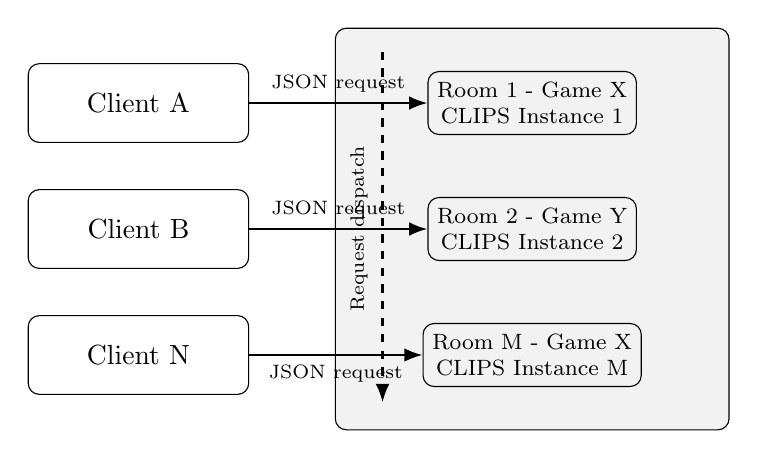
\begin{tikzpicture}[
  box/.style={draw, rounded corners, minimum width=2.8cm, minimum height=1.0cm, align=center},
  smallbox/.style={draw, rounded corners, minimum width=2.6cm, minimum height=0.8cm, align=center, font=\footnotesize},
  req/.style={-Latex, thick},
  flow/.style={-Latex, thick, dashed}
]

% Clients
\node[box] (c1) at (-5, 1.8) {Client A};
\node[box] (c2) at (-5, 0.2) {Client B};
\node[box] (c3) at (-5, -1.4) {Client N};

% Server
\node[box, minimum width=5.0cm, minimum height=5.1cm, fill=black!5] (server) at (0,0.2) {};

% Rooms and CLIPS instances inside server
\node[smallbox] (g1) at (0, 1.8) {Room 1 - Game X\\CLIPS Instance 1};
\node[smallbox] (g2) at (0, 0.2) {Room 2 - Game Y\\CLIPS Instance 2};
\node[smallbox] (g3) at (0, -1.4) {Room M - Game X\\CLIPS Instance M};

% Requests from clients
\draw[req] (c1.east) -- node[above, font=\scriptsize] {JSON request} (g1.west);
\draw[req] (c2.east) -- node[above, font=\scriptsize] {JSON request} (g2.west);
\draw[req] (c3.east) -- node[below, font=\scriptsize] {JSON request} (g3.west);

% Internal dispatch flow
\draw[flow] (-1.9, 2.45) -- (-1.9, -2.0);
\node[font=\scriptsize, rotate=90] at (-2.2, 0.2) {Request dispatch};

\end{tikzpicture}
\end{frame}

\begin{frame}{Prerequisites}
\begin{itemize}
  \item Git, subversion (for the repositories respectively of Rulemancer and CLIPS)
  \vspace{0.2cm}
  \item re2c 4.0+ (for CLIPS lexer generation)
  \vspace{0.2cm}
  \item Go 1.25+ (to build Rulemancer)
  \vspace{0.2cm}
  \item C compiler toolchain (to build CLIPS)
  \vspace{0.2cm}
  \item TLS certificate and key for HTTPS (self-signed is fine for testing)
  \vspace{0.2cm}
  \item JWT secret for runtime auth (\texttt{RULEMANCER\_JWT\_SECRET} or \texttt{--secret})
\end{itemize}
\end{frame}

\begin{frame}{Installation}
\begin{itemize}
\item Clone the repository:
\begin{block}{

git clone https://github.com/mmirko/rulemancer.git \\
cd rulemancer

}
\end{block}
\vspace{0.3cm}
  \item Clone/Install/Compile CLIPS with the provided script:
\begin{block}{

./install-clips.sh
}
\end{block}
\vspace{0.3cm}
  \item Build Rulemancer:
\begin{block}{

  make
}
\end{block}
\end{itemize}
\vspace{0.3cm}
The resulting binary will be located at \texttt{./rulemancer} \\
The games interface will be generated in \texttt{./interface}
\end{frame}



\begin{frame}{Configuration}
The server is configured via a JSON config file and/or runtime flags that can ovverride specific settings. \\
\vspace{0.5cm}
The default config file is \texttt{rulemancer.json} in the root directory, but an alternative path can be specified 
with \texttt{--config} flag. \\
\vspace{0.5cm}
Typical configuration options include:
\begin{itemize}
    \item \texttt{debug}, \texttt{debug\_level} (for logging verbosity)
    \item \texttt{engine\_port} (port for the API server)
    \item \texttt{tls\_cert\_file}, \texttt{tls\_key\_file} (paths to TLS certificate and key)
    \item \texttt{clipsless\_mode} (run without CLIPS integration for testing)
    \item \texttt{games} (e.g., \texttt{["rulepool"]}) to specify a set of CLIPS rule directories to load at startup
  \end{itemize}
\end{frame}

\begin{frame}{Running the Server}
To start the server, choose a secret for JWT authentication and set it either as an environment variable or via the
\texttt{--secret} flag and run the serve command:
\vspace{0.3cm}
\begin{itemize}
\item Using environment variable:
\begin{block}{
export RULEMANCER\_JWT\_SECRET="your-secret" \\
./rulemancer serve
}
\end{block}
\vspace{0.3cm}
\item With flag:
\begin{block}{
  ./rulemancer serve -secret="your-secret"
}
\end{block}
\end{itemize}
\vspace{0.3cm}
On startup, the engine prints an \textbf{admin JWT} that can be used for system-level operations and monitoring.
The server listens on the configured port (default: 3000) and serves the API under \texttt{/api/v1}. \\

\end{frame}


\begin{frame}{Tokens}
A script is provided to launch the server and capture the admin token in an environment variable for convenience:
\begin{block}{
source ./interface/[gameName]/launch.sh
}
\end{block}
Where \texttt{[gameName]} is the name of any game defined in \texttt{rulepool} (the script will be the same for all games
as they share the same server configuration). \\
\vspace{0.3cm}
Similarly, another script is provided to create a new client and capture its token:
\begin{block}{
source ./interface/[gameName]/client-create.sh
}
\end{block}
This will create a new client with a default name and description and store the returned \texttt{api\_token} 
in the \texttt{API\_TOKEN} environment variable for subsequent API calls.
\end{frame}


\begin{frame}[fragile]{Games}
  \begin{columns}
    \begin{column}{0.6\textwidth}
      Rulemancer supports multiple games running concurrently, each defined by a directory containing CLIPS rules and metadata.
      The configuration option \texttt{games} specifies which directories to load at startup. \\
      \vspace{0.4cm}
      Games cannot be added or removed at runtime, but multiple rooms of the same game can be created dynamically. \\
      \vspace{0.4cm}
      Each game must define a set of required CLIPS templates to establish the interface contract with the server.
    \end{column}
    \begin{column}{0.4\textwidth}
        \small
        \begin{verbatim}
(deftemplate game-config
  (slot game-name)
  (slot description)
  (slot num-players))

(deftemplate assertable
  (slot name)
  (multislot relations))

(deftemplate results
  (slot name)
  (multislot relations))

(deftemplate queryable
  (slot name)
  (multislot relations))
        \end{verbatim}
    \end{column}
  \end{columns}
\end{frame}

\begin{frame}{A game's Interface Contract in CLIPS}
To be recognized by Rulemancer, each game must define some CLIPS templates. The \texttt{game-config} template 
provides basic metadata about the game, its name, description, and number of players. \\
\vspace{0.3cm}
These other templates define the interface contract between the CLIPS rules and the server's API layer:
\begin{itemize}
  \item \texttt{assertable} defines accepted client actions (a.k.a. the moves or commands that players can perform).
  \item \texttt{results} defines the facts that will be returned to clients after processing a specific action.
  \item \texttt{queryable} defines any game state information that clients can query for at any time.
\end{itemize}
All of these templates use a flexible multislot to choose the specific relations inside the CLIPS environment.
\end{frame}

\begin{frame}{Interface built}
The subcommand \texttt{./rulemancer build} uses the aforementioned CLIPS templates to generate
additional interface files for each game, which are stored in the \texttt{interface/} directory. \\
\vspace{0.4cm}
These files are shell scripts that contain cURL commands for interacting with the server's API
according to the defined games and their assertable/queryable facts. \\
\vspace{0.4cm}
This allows developers to have a ready-made set of commands for testing and interacting with the server based
on the CLIPS rules they have defined, without needing to manually construct API requests. \\
\vspace{0.4cm}
The \texttt{make} command runs the build process automatically after compiling the server.
\end{frame}

% \begin{frame}{Interface built from CLIPS}
% Rulemancer automatically generates REST API endpoints based on the \texttt{assertable} and \texttt{queryable} templates defined in the CLIPS rules. \\
% \vspace{0.3cm}
% For each \texttt{assertable} fact, an endpoint of the form \texttt{/api/v1/room/\{id\}/assert/\{action\}} is created, where \texttt{\{action\}} corresponds to the name of the assertable fact. \\
% \vspace{0.3cm}
% Similarly, for each \texttt{queryable} fact, an endpoint of the form \texttt{/api/v1/room/\{id\}/query/\{query\}} is created. \\
% \vspace{0.3cm}
% This design allows game developers to define their game logic and API surface purely through CLIPS rules, without needing to write any additional server code for routing or request handling.
% \end{frame}

% \begin{frame}{Core Features}
% \begin{itemize}
%   \item CLIPS integration for inference and fact management.
%   \item Multi-game support from one server process.
%   \item Room isolation for concurrent matches.
%   \item Client + watcher model (players and spectators).
%   \item Dynamic web pages under \texttt{/api/v1/web/...}.
% \end{itemize}
% \end{frame}

% \begin{frame}{High-Level Architecture}
% \begin{itemize}
%   \item \textbf{Rule files} in \texttt{rulepool/} define game interface and behavior.
%   \item \textbf{Engine} loads games at startup and creates isolated room instances.
%   \item \textbf{API layer} maps HTTP endpoints to assert/query operations.
%   \item \textbf{WebSocket layer} broadcasts room activity in real time.
%   \item \textbf{Web client templates} render dynamic admin/game pages.
% \end{itemize}
% \end{frame}

% \begin{frame}{Repository Structure}
% \begin{itemize}
%   \item \texttt{cmd/} $\rightarrow$ CLI commands (\texttt{serve}, \texttt{build}, \texttt{test}).
%   \item \texttt{pkg/rulemancer/} $\rightarrow$ engine, API handlers, monitor/websocket, templating.
%   \item \texttt{core/} $\rightarrow$ CLIPS C sources and headers.
%   \item \texttt{rulepool/} $\rightarrow$ game rules + metadata (\texttt{*.clp}).
%   \item \texttt{testpool/} $\rightarrow$ CLIPS test facts/scenarios.
% \end{itemize}
% \end{frame}





% \begin{frame}{CLI Workflow}
% \begin{itemize}
%   \item \texttt{./rulemancer test} $\rightarrow$ load \texttt{rulepool/} + \texttt{testpool/} into CLIPS and run checks.
%   \item \texttt{./rulemancer build} $\rightarrow$ generate extra interfaces (default output: \texttt{interface/}).
%   \item \texttt{./rulemancer serve} $\rightarrow$ launch HTTPS API + web routes.
%   \item Simple dev cycle: \textbf{edit rules $\rightarrow$ test $\rightarrow$ build extras $\rightarrow$ serve}.
% \end{itemize}
% \end{frame}

% \begin{frame}{Security Model (JWT)}
% \begin{itemize}
%   \item New clients are created without auth: \texttt{POST /api/v1/new/client}.
%   \item Response returns \texttt{id} and \texttt{api\_token}.
%   \item All protected routes require:
%   \begin{itemize}
%     \item \texttt{Authorization: Bearer <token>}
%   \end{itemize}
%   \item Admin token is required for system operations (health/quit/system WS).
% \end{itemize}
% \end{frame}

% \begin{frame}{API Overview}
% \begin{itemize}
%   \item \texttt{/system} $\rightarrow$ health, shutdown, system websocket.
%   \item \texttt{/client} $\rightarrow$ list, current, details, delete.
%   \item \texttt{/game} $\rightarrow$ list and game metadata.
%   \item \texttt{/room} $\rightarrow$ create/list/get/delete + assert/query/ws.
%   \item \texttt{/join} and \texttt{/watch} $\rightarrow$ room participation workflows.
% \end{itemize}
% \end{frame}

% \begin{frame}{Typical Player Journey}
% \begin{enumerate}
%   \item \texttt{POST /new/client} to obtain token.
%   \item Join game (\texttt{/join/available/\{game\}} or \texttt{/join/new/\{game\}}).
%   \item Assert actions (\texttt{/room/\{id\}/assert/\{action\}}).
%   \item Query state (\texttt{/room/\{id\}/query/\{query\}}).
%   \item Subscribe to room websocket for live updates.
% \end{enumerate}
% \end{frame}

% \begin{frame}{Game and Room Endpoints (Examples)}
% \begin{itemize}
%   \item List games: \texttt{GET /api/v1/game/list}
%   \item Inspect game schema: \texttt{GET /api/v1/game/\{id\}}
%   \item Create room: \texttt{POST /api/v1/room/create}
%   \item List rooms: \texttt{GET /api/v1/room/list}
%   \item Inspect room: \texttt{GET /api/v1/room/\{id\}}
% \end{itemize}
% \end{frame}

% \begin{frame}{Assert and Query Endpoints}
% \begin{itemize}
%   \item Assert action:
%   \begin{itemize}
%     \item \texttt{POST /api/v1/room/\{id\}/assert/move}
%   \end{itemize}
%   \item Query state:
%   \begin{itemize}
%     \item \texttt{POST /api/v1/room/\{id\}/query/cell}
%     \item \texttt{POST /api/v1/room/\{id\}/query/winner}
%   \end{itemize}
%   \item Response envelope format: \texttt{\{ "response": \{ ... \} \}}
% \end{itemize}
% \end{frame}

% \begin{frame}{Real-Time Communication}
% \begin{itemize}
%   \item System monitor websocket:
%   \begin{itemize}
%     \item \texttt{wss://localhost:3000/api/v1/system/ws} (admin)
%   \end{itemize}
%   \item Room websocket:
%   \begin{itemize}
%     \item \texttt{wss://localhost:3000/api/v1/room/\{id\}/ws}
%   \end{itemize}
%   \item Trigger model: each assert broadcasts room notifications to connected clients/watchers.
% \end{itemize}
% \end{frame}


% \begin{frame}{Example: Tic-Tac-Toe}
% \begin{itemize}
%   \item Assertable: \texttt{move}
%   \item Results relation: \texttt{last-move}
%   \item Queryables: \texttt{winner}, \texttt{cell}
%   \item Demonstrates complete flow from action submission to board/winner retrieval.
% \end{itemize}
% \end{frame}

% \begin{frame}{Web Interface (Built-In)}
% \begin{itemize}
%   \item Route family mounted at \texttt{/api/v1/web}.
%   \item Dynamic pages are generated from templates at startup.
%   \item Admin page and game-specific client pages are served directly by backend.
%   \item Example game page path: \texttt{/api/v1/web/client/\{gameName\}}.
% \end{itemize}
% \end{frame}

% \begin{frame}{Admin Dashboard Capabilities}
% \begin{itemize}
%   \item Login with admin JWT.
%   \item Browse games, rooms, and clients.
%   \item Inspect object details and payloads.
%   \item Connect to room websockets for live monitoring.
%   \item Operational controls include server-oriented actions.
% \end{itemize}
% \end{frame}

% \begin{frame}{Game Client Page Capabilities}
% \begin{itemize}
%   \item Enter JWT + room context.
%   \item Render assert forms from game protocol data.
%   \item Trigger query actions and view structured responses.
%   \item Open websocket stream for live room events.
%   \item Useful for rapid prototyping and debugging game interfaces.
% \end{itemize}
% \end{frame}

% \begin{frame}{Demo Flow, Limits, and Next Steps}
% \begin{itemize}
%   \item \textbf{Live demo sequence:}
%   \begin{enumerate}
%     \item Start server and capture admin token.
%     \item Create two clients and join a room.
%     \item Execute moves via API/web page.
%     \item Observe real-time websocket updates.
%   \end{enumerate}
%   \item \textbf{Current strengths:} rule-driven extensibility, room isolation, real-time monitoring.
%   \item \textbf{Next steps:} richer frontend UX, stronger authorization policies, packaged deployment profiles.
% \end{itemize}
% \end{frame}

% \begin{frame}[fragile]{Appendix A — Useful cURL Snippets}
% \textbf{Create client}
% \begin{verbatim}
% curl -k -X POST https://localhost:3000/api/v1/new/client \
%   -H "Content-Type: application/json" \
%   -d '{"name":"Alice","description":"Player"}'
% \end{verbatim}

% \textbf{Join available room}
% \begin{verbatim}
% curl -k -X POST https://localhost:3000/api/v1/join/available/tictactoe \
%   -H "Authorization: Bearer $API_TOKEN"
% \end{verbatim}

% \textbf{Assert move}
% \begin{verbatim}
% curl -k -X POST https://localhost:3000/api/v1/room/$ROOM_ID/assert/move \
%   -H "Authorization: Bearer $API_TOKEN" \
%   -H "Content-Type: application/json" \
%   -d '{"move":[{"x":["1"],"y":["1"],"player":["x"]}]}'
% \end{verbatim}
% \end{frame}

% \begin{frame}{Appendix B — Error Model and HTTP Statuses}
% \begin{itemize}
%   \item Error body format: \texttt{\{ "error": "message" \}}
%   \item Common statuses: \texttt{200}, \texttt{201}, \texttt{400}, \texttt{401}, \texttt{404}, \texttt{409}, \texttt{500}
%   \item Recommended client behavior: handle auth expiration, retry idempotent reads, surface server message for debugging.
% \end{itemize}
% \end{frame}

\end{document}
